\subsection{Moving obstacle}
We look at a motion planning problem shown in figure \ref{fig:exp1} where the agent is tasked with reaching the goal state in green whilst avoiding collisions with the red static obstacles and an orange moving obstacle that moves in the area shown. This is expressed in LTL as $\LTLdiamond \lnot$'crash' $\wedge$  $\LTLdiamond$'goal'. Where the atomic proposition 'crash' is true in the red static obstacles or when the state of the agent is the same as the state of the moving obstacle. The atomic proposition 'goal' is true in the green cell. The DFA representation is shown in Figure \ref{fig:dra}.
\begin{figure}
\subfloat[Gridworld with moving obstacle \label{fig:exp1}]{
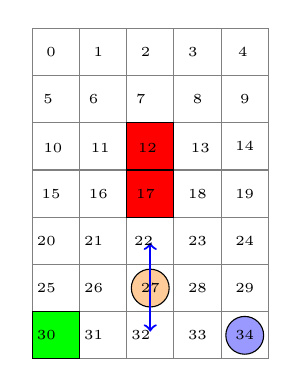
\begin{tikzpicture}[scale=1.2]
\draw[step=0.5cm,color=gray] (-1.5,-2.5) grid (1,1);
\filldraw[fill=red,draw=black] (0,0) rectangle (-0.5,-0.5);
\filldraw[fill=red,draw=black] (0,-0.5) rectangle (-0.5,-1);
\filldraw[fill=green,draw=black] (-1.5,-2.5) rectangle (-1,-2.0);
\filldraw[fill=blue!40!white,draw=black] (+0.75,-2.25) circle (0.2cm);
\filldraw[fill=orange!40!white,draw=black] (-0.25,-1.75) circle (0.2cm);
\draw[blue,thick,->] (-0.25,-1.73) -> (-0.25,-1.27);
\draw[blue,thick,->] (-0.25,-1.73) -> (-0.25,-2.21);
\node at (-1.30,+0.75) {\tiny{0}};
\node at (-0.80,+0.75) {\tiny{1}};
\node at (-0.30,+0.75) {\tiny{2}};
\node at (0.20,+0.75) {\tiny{3}};
\node at (0.73,+0.75) {\tiny{4}};
\node at (-1.33,+0.25) {\tiny{5}};
\node at (-0.85,+0.25) {\tiny{6}};
\node at (-0.35,+0.25) {\tiny{7}};
\node at (0.25,+0.25) {\tiny{8}};
\node at (0.75,+0.25) {\tiny{9}};
\node at (-1.28,-0.27) {\tiny{10}};
\node at (-0.78,-0.27) {\tiny{11}};
\node at (-0.28,-0.27) {\tiny{12}};
\node at (0.28,-0.27) {\tiny{13}};
\node at (0.75,-0.25) {\tiny{14}};
\node at (-1.3,-0.75) {\tiny{15}};
\node at (-0.8,-0.75) {\tiny{16}};
\node at (-0.3,-0.75) {\tiny{17}};
\node at (0.25,-0.75) {\tiny{18}};
\node at (0.75,-0.75) {\tiny{19}};
\node at (-1.35,-1.25) {\tiny{20}};
\node at (-0.85,-1.25) {\tiny{21}};
\node at (-0.32,-1.25) {\tiny{22}};
\node at (0.25,-1.25) {\tiny{23}};
\node at (0.75,-1.25) {\tiny{24}};
\node at (-1.35,-1.75) {\tiny{25}};
\node at (-0.85,-1.75) {\tiny{26}};
\node at (-0.25,-1.75) {\tiny{27}};
\node at (0.25,-1.75) {\tiny{28}};
\node at (0.75,-1.75) {\tiny{29}};
\node at (-1.35,-2.25) {\tiny{30}};
\node at (-0.85,-2.25) {\tiny{31}};
\node at (-0.35,-2.25) {\tiny{32}};
\node at (0.25,-2.25) {\tiny{33}};
\node at (0.75,-2.25) {\tiny{34}};
\end{tikzpicture}
}
\subfloat[Specification DFA\label{fig:dra}]{
	\begin{tikzpicture}[shorten >=1pt,node distance=1.6cm,on grid]
	\node[state,initial]   (q_0)                {$s_0$};
	\node[state,accepting]           (q_1) [right=of q_0] {$s_1$};
	\node[state] (q_2) [below=of q_1] {$s_2$};
	\path[->] (q_0) edge                node [above] {\small Goal} (q_1)
	edge [loop above]   node         {} ()
	%edge [bend left=45] node [below] {1} (q_2)
	edge [bend right]   node [left] {\small Crash} (q_2)
	(q_1) edge                node [right] {\small Crash} (q_2)
	edge [loop above]         node {} (q_1)
	(q_2) edge [loop below]   node {} (q_2);
	\end{tikzpicture}
}
\caption{Gridworld and DFA  with $\textrm{Acc}_{\mathcal{M}} = (s_1)$ depicting a scenario where agent in blue has to reach green target cell without crashing into the red static obstacles or the orange moving obstacle.}\label{fig:exp2}
\end{figure}

The state space of the agent is $(x,y,x_{obs},y_{obs})$ where $(x_{obs},y_{obs})$ form the position of the moving obstacle. We assume that the state of the moving obstacle to be expensive to observe. Formally, we let $\mathcal{\tilde{X}} = (x,y)$ and $\mathcal{\bar{X}} = (x_{obs},y_{obs})$. 

 Intuitively we expect to see if that we set the $\beta$ parameter high, \ie if the cost of information is high, the agent will go the long way around the wall as it will be too expensive to observe the moving obstacle. Howver, if the agent knows the position of the moving obstacle at all times, it can easily plan to avoid collision, and hence for low $\beta$, we expect to see the agent go through shorter route. We use a time horizon $T = 25$ and test for $\beta = 0.5$ and $\beta=5$

\begin{figure}
	\subfloat[$\beta = 0.5$\label{simple-grid}]{
	\includegraphics[scale=.5]{lowbb}}
	%\hfill
	\subfloat[$\beta = 5$\label{fig:simple-transitions}]{
		\includegraphics[scale=0.5]{highb}
	}
	\caption{Probability distribution of the agent after 16/25 timesteps. a) has a low $\beta$ which means information cost is low while b) has a high $\beta$ and hence high cost on information}
	\label{fig:expres}
\end{figure}

Figure \ref{fig:expres} shows the probability distributions of the agent at a specific time $t=16$. Clearly, in the case where $\beta=0.5$, the agent is able to go through the region where the moving obstacle operates. However, when we increase the cost of information, the agent moves around the static obstacles.

